\section{Microcontroller}

\subsection{OS}
\subsection{Scheduling}
\subsection{Tasks}

\subsubsection{Uart}

Uart står for universal asynchronous receiver/transmitter. Dette laver kommunikation mellem to enheder. Så være enhed skal være i stand til at bruge funktion UART. UART transmittere data i form af bytes og deler dem op i bits og sender dem. Modtager skal så kunne samle dem sammen igen til bytes for at læse det.
Vores Uart pinde sider på PORT A, derved skal sysctl aktiveres på port a før den viker. Uart har en init. funktion som bliver kaldt en gang hvor alle register bliver sat up som, f.eks. send og modtag. Der bliver også sat en baut rate, som skal være den samme for sender og modtager.
\\
For at sende data kalder vi funktion uart0\textunderscore putc som tager en karakter. Dette kan både være tal og bogstaver. Der en funktion der hedder uart0\textunderscore rx\textunderscore rdy som venter på at den modstager noget.
\\
Uart er en god måde til at sende information når man f.eks. skal debugge eller vil have nogen bestemte data hen til ens computer.

\subsubsection{LCD}

Til vores kit er der givet et liqiud-crystal display (LCD), som har størrelsen 2x16. For at kunne bruge dette display, som er på PORT C og PORT D, der skal aktiveres ved hjælp at sysctl før det kan bruges. For at sende sætte LCD’ed i forskellige mods skal det gøres på PORT C og sende data. Den har RS og E på PORT D.
\\
Dette display har to modes 8 bit og 4 bit, fordi fire af vores pinde er sat til ground kan den kun køre 4 bit mode.
LCD modulet har nogen forskellige funktioner, dem der bliver brugt oftes er wr\textunderscore str\textunderscore LCD, som laver en pointer og sender de enkelte karaktere ud en efter en, ved hjælp af funktion wr\textunderscore ch\textunderscore LCD. Disse funktion er til for at gøre det simpelt for at sende noget. De bliver sendt ind i en funktion som gør at karakteren bliver skrevet ud til PORT C data register og herefter bliver mode sat i PORT D data register.

\subsubsection{Keypad}

Keypad
I vores Kit er der givet en keypad med 12 knapper fra 0 til 9 og *,\#. Dette keypad virker bare som switches så derfor skal vi selv definere hvad de forskellige knapper skal gøre, for at gøre det simpelt betyder hver knap det som der står på keypaded. Den har to porte til knyttet som er PORT A og PORT E. Det betyder at vi kan læse på PORT E hvis en af GPIO pinden på PORT A er aktiv. [Billede Keypad]
\\
Dette billede kan vi se at vi har givet de forskellige knapper unikke værdier. Dette gøre fordi vi har et array som indeholder alle værdier på keypad’et, som vi så sender kan sende ind i buffer og læse på. For at finde en karakter kigger vi først på alle X værdier (PORT A) igennem og ser om en Y værdi (PORT E) er aktiv og ud fra hvilken X og Y værdi fordi en af tallen på  [Ref billede Keypad].
\\
Dette keypad kan blive brugt til at sende data eller manuelt vil sætte nogle værdier i mens programmet køre.




\subsection{Serial Peripheral Interface}

Microcontrolleren der blev udleveret dette semester (TM4C123GH6PM) indeholder 4 SSI (Synchronous Serial Interface) da disse 4 interfaces alle er ens, på undtagelse deres pins, er SSI0 blevet valgt som interface, dvs. port A pin 2 er til SSI0Clk (modulets clock), pin 3 er SSI0Fss (frame signalet), pin 4 er SSI0Rx (modtagelse), og pin 5 er SSI0Tx (afsendelse)

Til SSI modulet er der 3 forskellige data formater:

\begin{itemize}
	\item Texas Instruments Synchronous Serial
		\begin{figure}[h]
			\begin{center}
			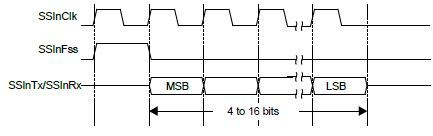
\includegraphics[scale=1]{Billeder/TI_Synchronous_Serial_Frame_Format.jpg}
			\end{center}
			\label{fig:TIFrameFormat}
			\caption{TI Synchronous Serial Frame Format (Single transfer)}
		\end{figure}

	\item Freescale SPI
		\begin{figure}[h]
			\begin{center}
			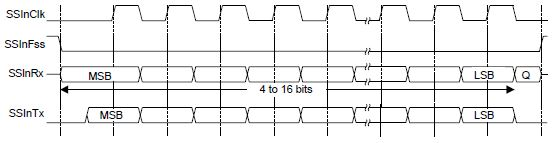
\includegraphics[scale=1]{Billeder/FS_Frame_Format.jpg}
			\end{center}
			\label{fig:FSFrameFormat}
			\caption{FreeScale Frame Format (Single Transfer)}
		\end{figure}
		  
	\item Microwire
		\begin{figure}[h]
			\begin{center}
			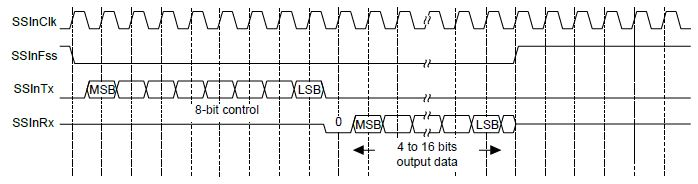
\includegraphics[scale=0.8]{Billeder/MW_Frame_format.jpg}
			\end{center}
			\label{fig:MWFrameFormat}
			\caption{Micro Wire Frame Format (Single Transfer)}
		\end{figure}
\end{itemize}